\documentclass[class=report,crop=false, 12pt]{standalone}
\usepackage[screen,nosolutions]{../scratch}

\begin{document}

\titre[S]{Invasion}
%===============================

\insertvideo{y0yXDazTiMc}{Invasion -- Activité 1}

\insertvideo{eUZnarcEx7w}{Invasion -- Activité 2}

\insertvideo{50VkJkhHTlw}{Invasion -- Activité 3}

\bigskip
\bigskip


Tu vas programmer en trois étapes un jeu s'inspirant du célèbre jeu \emph{Space invaders}.

\begin{center}
  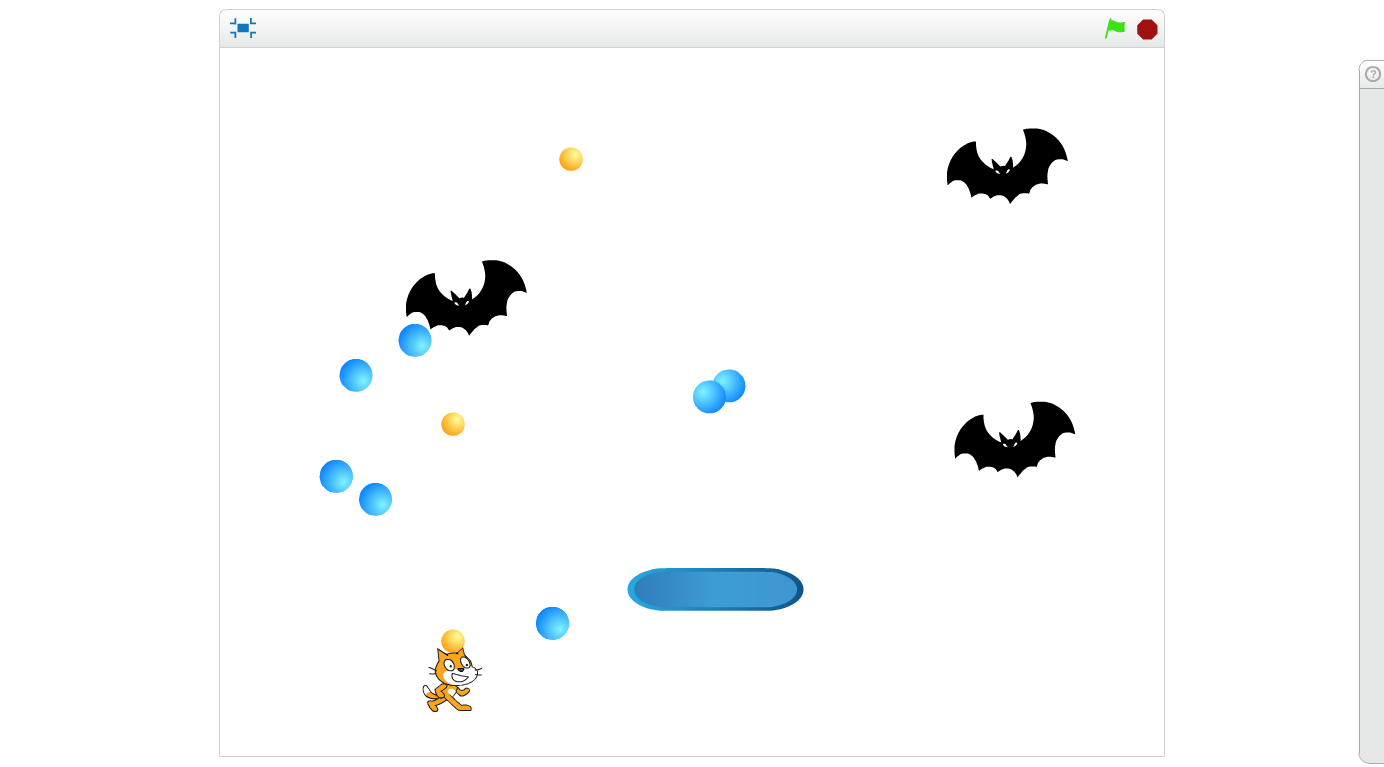
\includegraphics[scale=\scaleecran]{ecran-10-ex0} 
\end{center}

Le chat est attaqué par des chauves-souris qui lui lancent des bombes bleues. Il réplique avec des balles jaunes. Le chat peut aussi s'abriter sous un abri, mais celui-ci n'est que provisoire. 

\begin{activite}[Le chat et les balles]

Programme le chat qui lance des balles.
\begin{itemize}
  \item Le chat se déplace vers la droite ou la gauche avec les touches de flèches.
  \item Si la touche de la flèche vers le haut est pressée, alors le chat lance une balle.
  \item Chaque balle part du chat et monte verticalement.
\end{itemize}


\begin{center}
  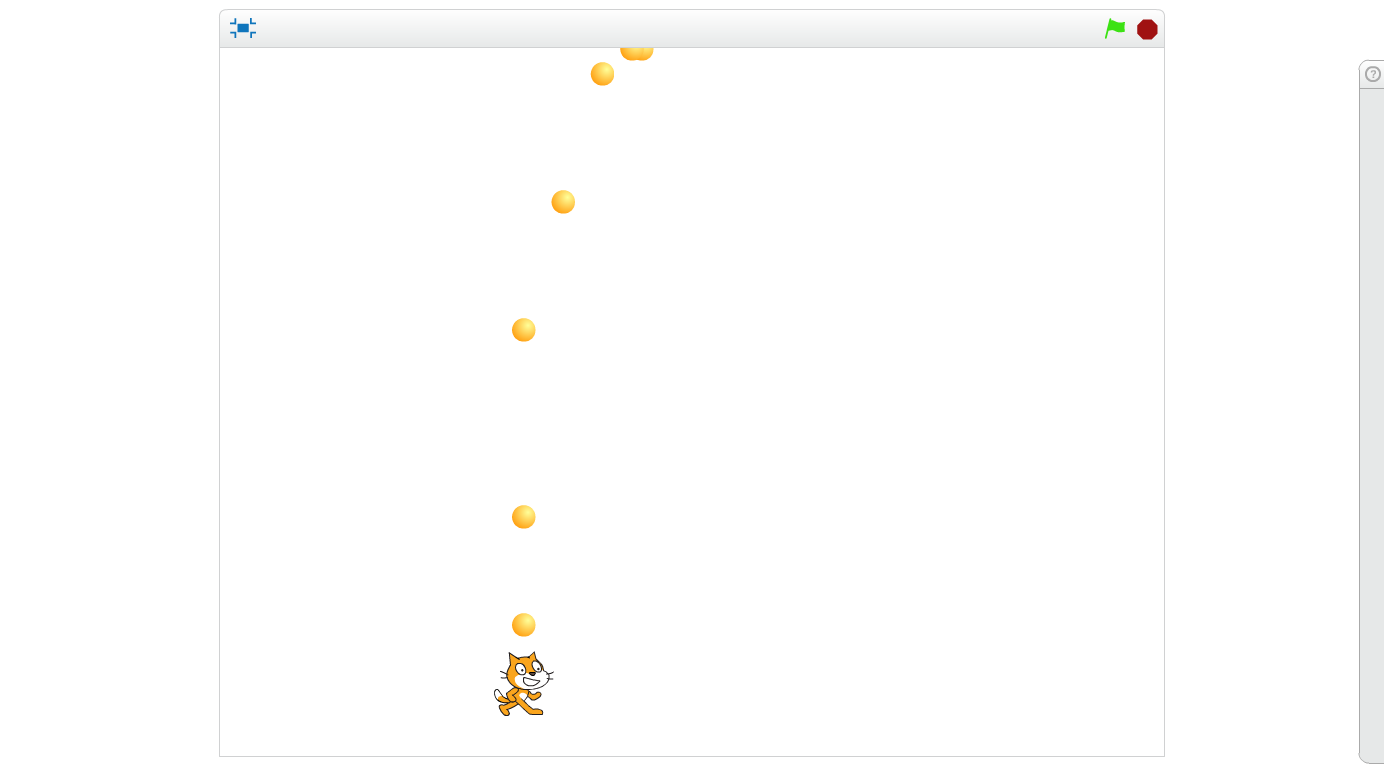
\includegraphics[scale=\scaleecran]{ecran-10-ex1} 
\end{center}


\bigskip

\textbf{Les balles clonées.}

Comment lancer plusieurs balles ? Il suffit d'écrire le programme pour une seule balle et de créer des clones !
\begin{itemize}
  \item Pour lancer une balle, le chat exécute l'instruction  \og Créer un clone de balle \fg{}.
  \item Le code pour la balle commence par \og quand je commence comme un clone \fg{} (au lieu de \og quand le drapeau vert est cliqué \fg{}).
\end{itemize}

\bigskip

\textbf{Blocs utiles.}

\begin{center}
  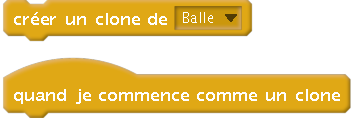
\includegraphics[scale=\scalebloc]{bloc-10-ex1} 
\end{center} 
  
\end{activite}



\begin{activite}[La chauve-souris attaque]

\sauteligne

\begin{itemize}
  \item La chauve-souris se déplace de droite à gauche et de gauche à droite.
  \item Si elle est touchée par une balle du chat, c'est terminé pour elle (cache-la et arrête son script).
  \item De temps en temps elle lance une bombe (par exemple, tire au hasard un nombre entre $1$ et $20$, si ce nombre est $1$, lance une bombe, puis attends un peu avant de tirer un autre nombre au hasard).
  \item Cette fois encore, la bombe est un nouveau clone, créé par la chauve-souris.
  \item La bombe s'oriente à $180$\textdegree\ et descend verticalement.
  \item Modifie le script du chat. S'il est touché par une bombe, c'est perdu : joue un son et arrête tout.
\end{itemize}

\begin{center}
  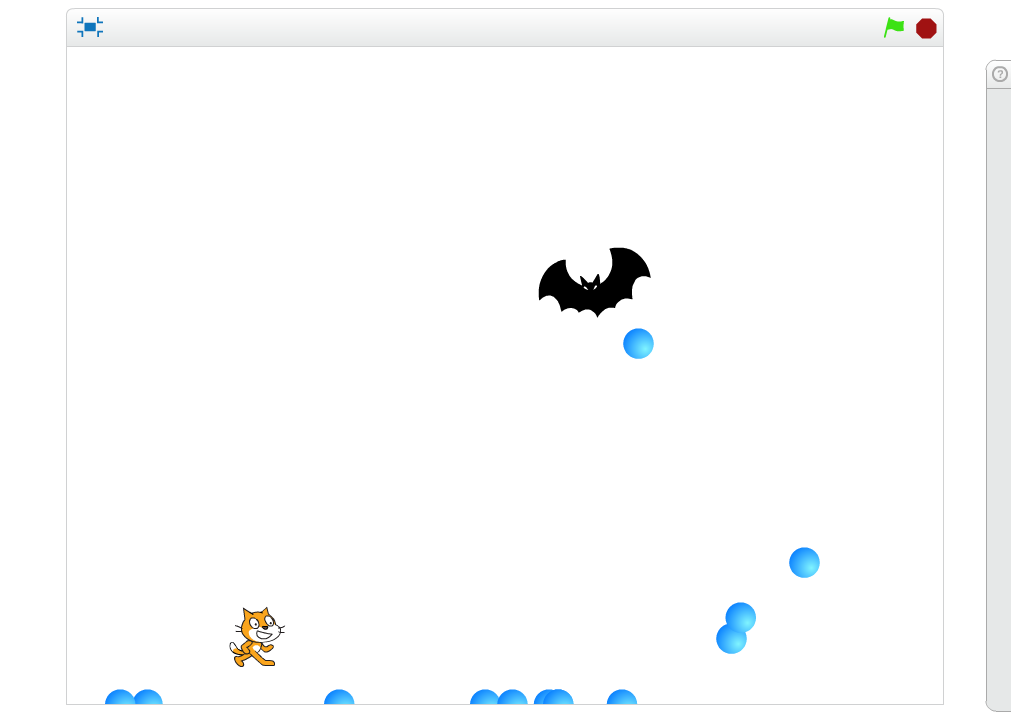
\includegraphics[scale=\scaleecran]{ecran-10-ex2} 
\end{center}

  
\end{activite}


\begin{activite}[Un pare-bombes]

Protège le chat avec un pare-bombes. Celui-ci disparaîtra après avoir reçu $5$ bombes.
\begin{itemize}
  \item Le pare-bombes possède $5$ vies. Chaque fois qu'une bombe le touche, il perd une vie. Lorsqu'il n'a plus de vie, il disparaît.
  
  \item Si une bombe tombe sur le pare-bombes, elle repart vers le haut.

  \item Si une balle, lancée par le chat, touche le pare-bombes, elle disparaît.
\end{itemize}


\begin{center}
  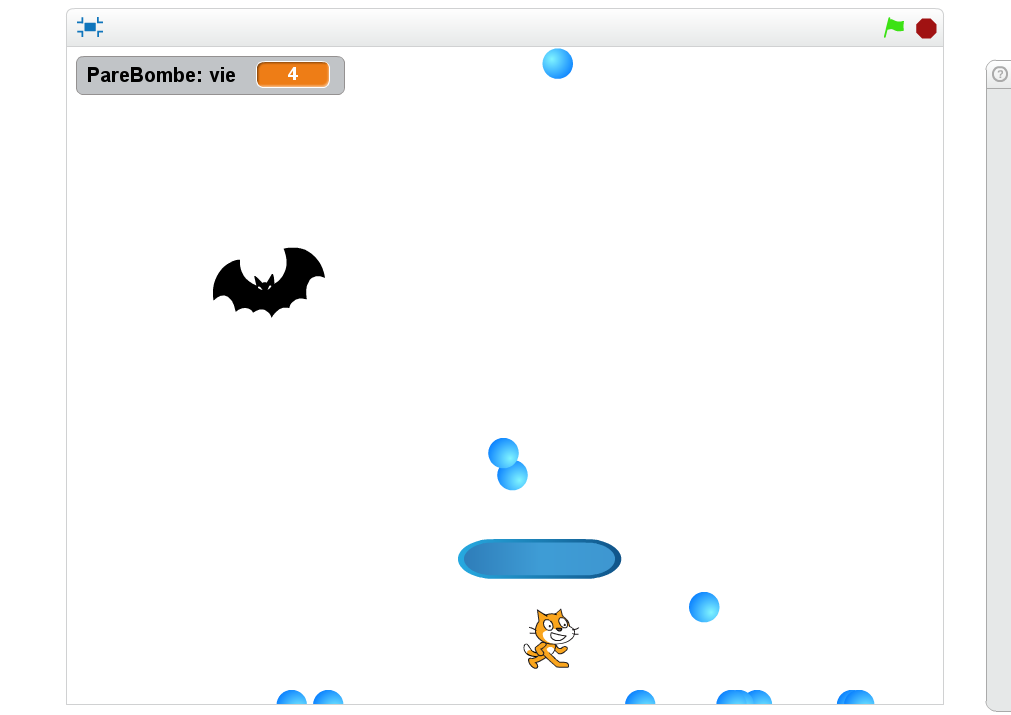
\includegraphics[scale=\scaleecran]{ecran-10-ex3} 
\end{center}


\textbf{Bonus}

\begin{itemize}
  \item Duplique la chauve-souris pour augmenter la difficulté.
  
  \item Rajoute d'autres pare-bombes pour aider le chat.
  
  \item Affiche un score, rajoute des vies au chat...

\end{itemize}
  
\end{activite}




\ifx \displaysolutions \myzero
\else
\begin{code}
\onesolution{Invasion}{Activité 1}{
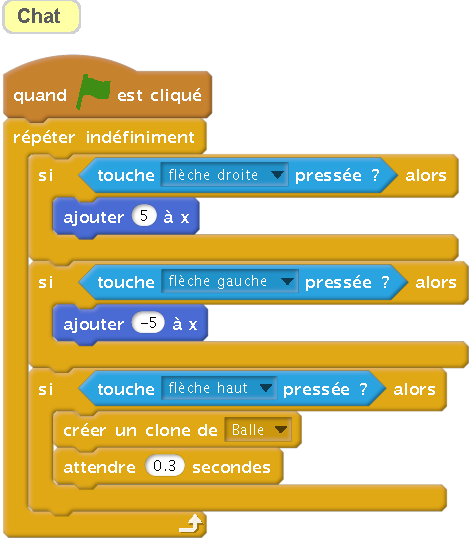
\includegraphics[scale=\scalesolution]{code-10-ex1a}
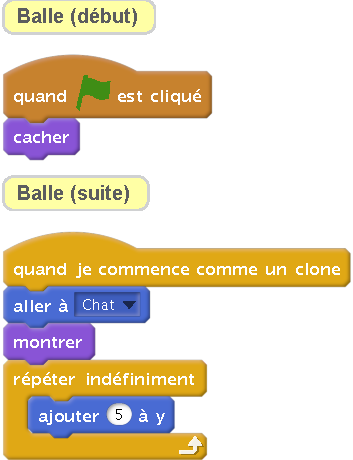
\includegraphics[scale=\scalesolution]{code-10-ex1b}
}
\onesolution{Invasion}{Activité 2}{
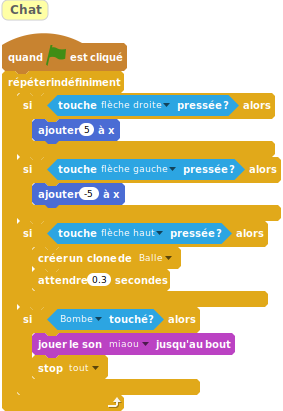
\includegraphics[scale=\scalesolution,scale=0.75]{code-10-ex2a}
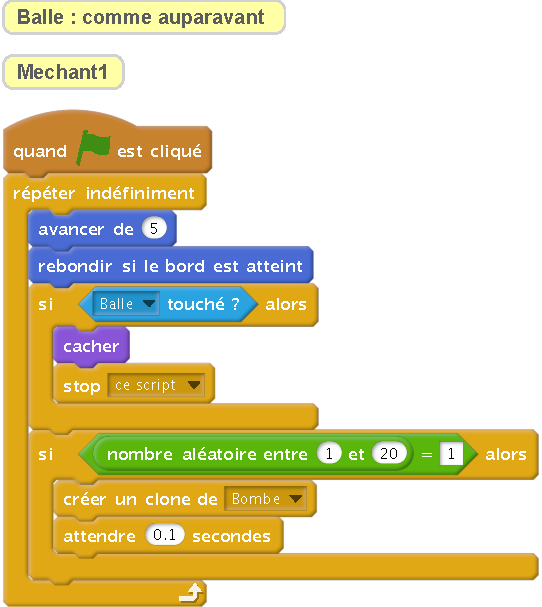
\includegraphics[scale=\scalesolution,scale=0.75]{code-10-ex2b}
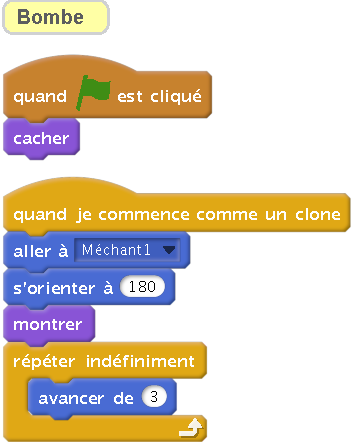
\includegraphics[scale=\scalesolution,scale=0.75]{code-10-ex2c}
}
\onesolution{Invasion}{Activité 3}{
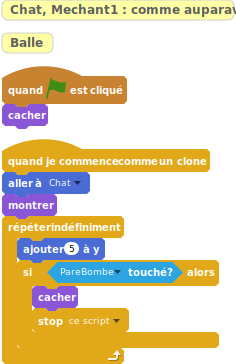
\includegraphics[scale=\scalesolution,scale=0.9]{code-10-ex3a}
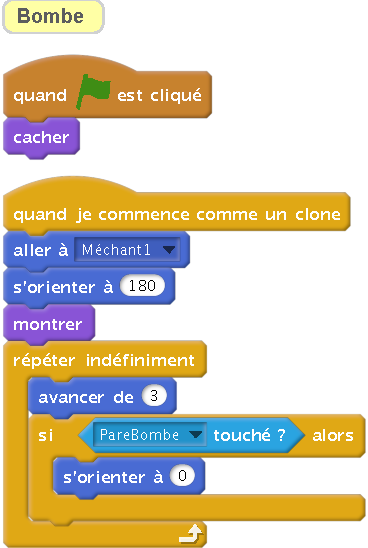
\includegraphics[scale=\scalesolution,scale=0.9]{code-10-ex3b}
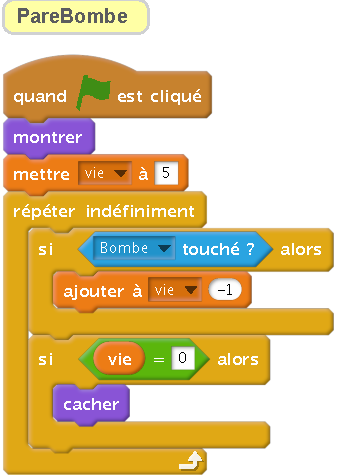
\includegraphics[scale=\scalesolution,scale=0.9]{code-10-ex3c}
}    
\end{code}
\fi

\end{document}

